


In diesem Abschnitt sind aktuell einige Unterlagen eingefügt, die im Rahmen des Projektes eine Relevanz hatten. Vor Abgabe der Projektarbeit, soll dieser Abschnitt überarbeitet, ausgedünnt und ergänzt werden. 

\section{Projektnotizen}

Austausch und Zusammenarbeite erfolgte auf verschiedenen Platformen:
\begin{itemize}
    \item Gezeichnet und Entwürfe wurden meist in Miro erstellt: \url{https://miro.com/app/board/uXjVOdN2haQ=/}. 
    \item Besprechungen erfolgten meist in Teams: \url{https://teams.microsoft.com/l/team/19%3aDoBvOwOIC6WNhsL9kOIYFKNtVftU1yBtcEn_gcyQtcg1%40thread.tacv2/conversations?groupId=850a22ff-34a2-4fe2-a506-f55ac4d595f8&tenantId=b9b6f99a-a243-422d-ab36-f726574c981a}. 
    \item Der gemeinsame Code und die Dokumentation wurden auf Github erstelt: \url{https://github.com/tstsrv-de/tstsrv-de}. 
\end{itemize}

\subsection{Projektbesprechungen}

Stets Sonntags erfolgten Projektbesprechungen. Notizen und Zusammenfassungen davon finden sich hier in fortschreitender, chronologischer Reihenfolge. Ebenso hier entsprechend einsortiert, finden sich Konzeptzeichnungen und Entwürfe aller Art (UI, Code, Datenbankmodelle).

(TODO!) Bildbeschreibungen ergänzen, wichtige Bilder beschreiben.

2021-11-23-erster-entwurf-gameloop 
\begin{figure}[H]
    \centering
    \caption[]{2021-11-23-erster-entwurf-gameloop}
    \label{fig:2021-11-23-erster-entwurf-gameloop}
    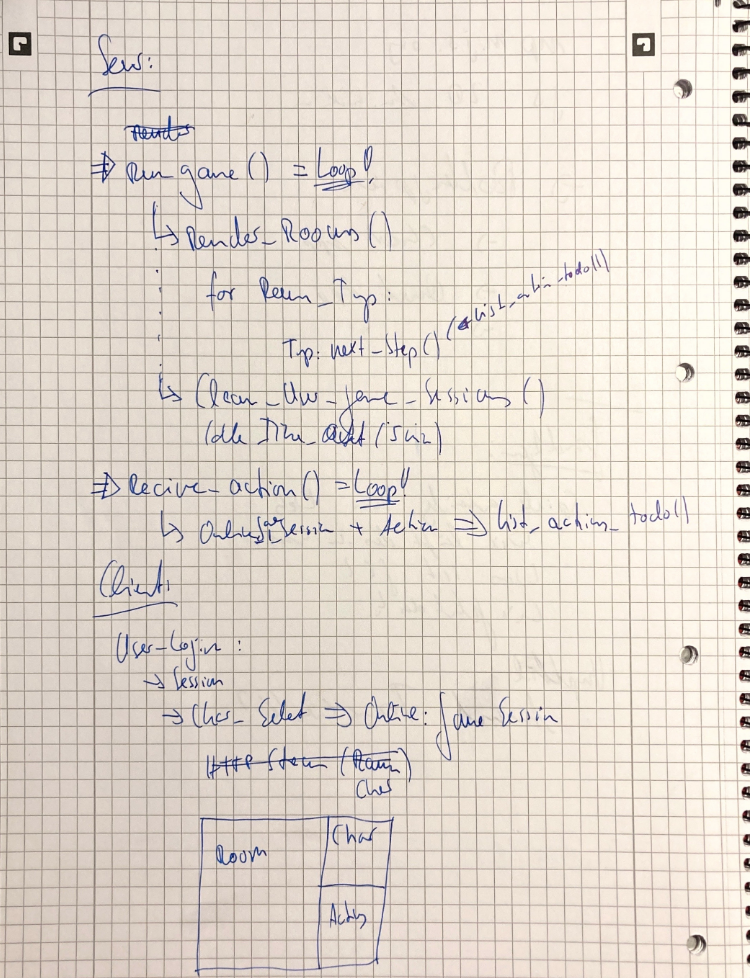
\includegraphics[width=1\textwidth]{2021-11-23-erster-entwurf-gameloop}
\end{figure}

2021-11-23-erstes-db-konzept 
\begin{figure}[H]
    \centering
    \caption[]{2021-11-23-erstes-db-konzept}
    \label{fig:2021-11-23-erstes-db-konzept}
    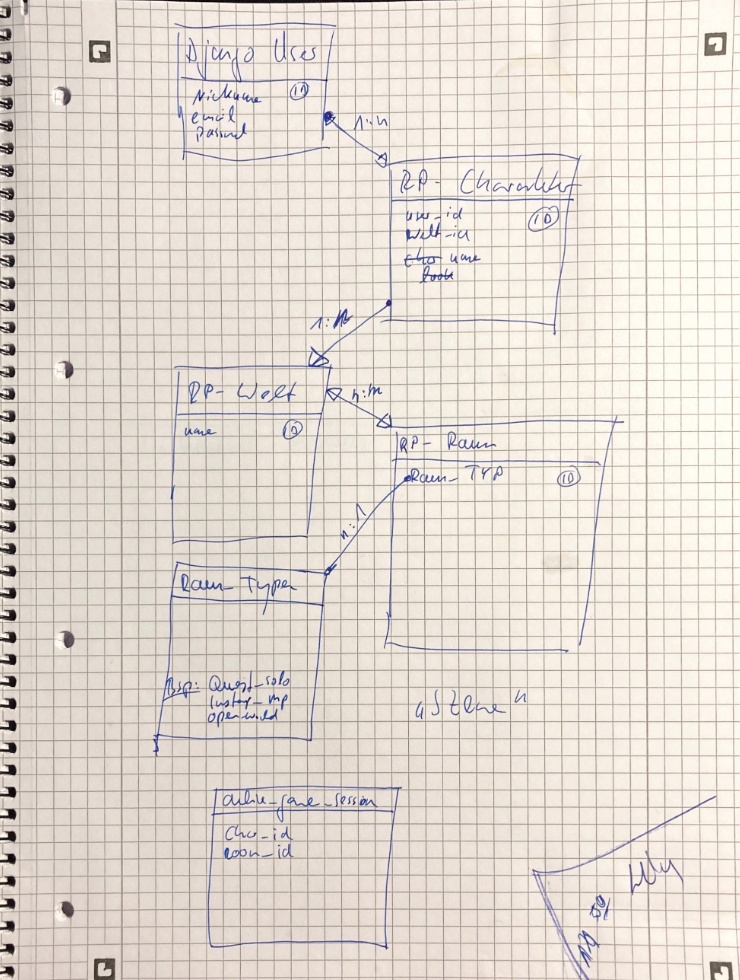
\includegraphics[width=1\textwidth]{2021-11-23-erstes-db-konzept}
\end{figure}

2021-11-27-erstentwurf-ui 
\begin{figure}[H]
    \centering
    \caption[]{2021-11-27-erstentwurf-ui}
    \label{fig:2021-11-27-erstentwurf-ui}
    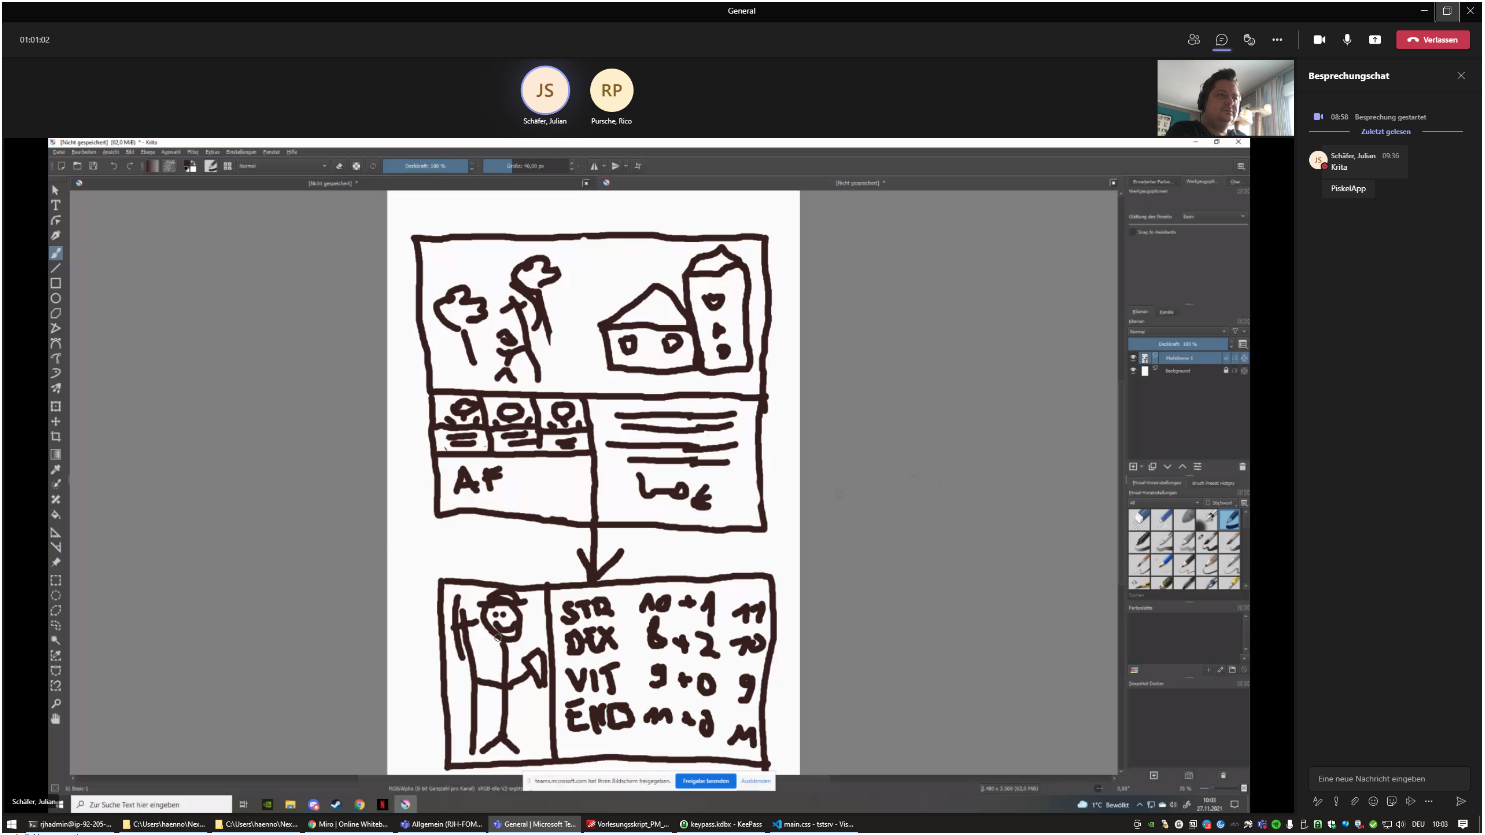
\includegraphics[width=1\textwidth]{2021-11-27-erstentwurf-ui}
\end{figure}

2021-11-27-projektskizze-1 
\begin{figure}[H]
    \centering
    \caption[]{2021-11-27-projektskizze-1}
    \label{fig:2021-11-27-projektskizze-1}
    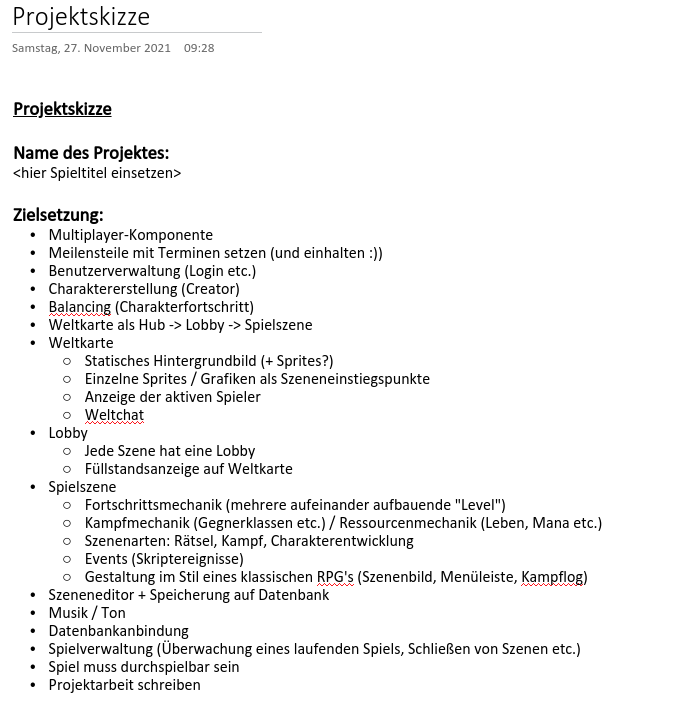
\includegraphics[width=1\textwidth]{2021-11-27-projektskizze-1}
\end{figure}

2021-11-27-projektskizze-2 
\begin{figure}[H]
    \centering
    \caption[]{2021-11-27-projektskizze-2}
    \label{fig:2021-11-27-projektskizze-2}
    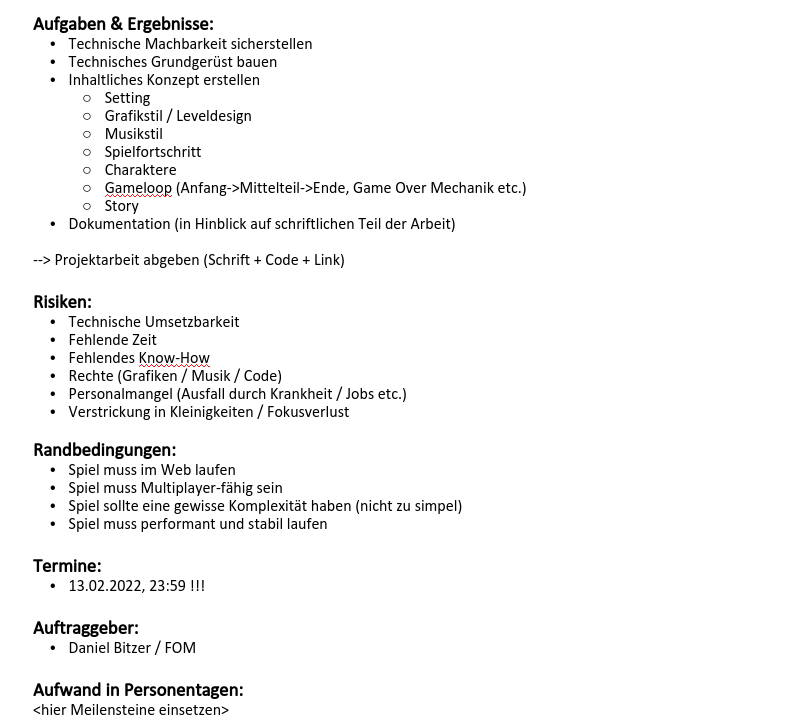
\includegraphics[width=1\textwidth]{2021-11-27-projektskizze-2}
\end{figure}

2021-11-29-Entwurf-Klassen-Ui 
\begin{figure}[H]
    \centering
    \caption[]{2021-11-29-Entwurf-Klassen-Ui}
    \label{fig:2021-11-29-Entwurf-Klassen-Ui}
    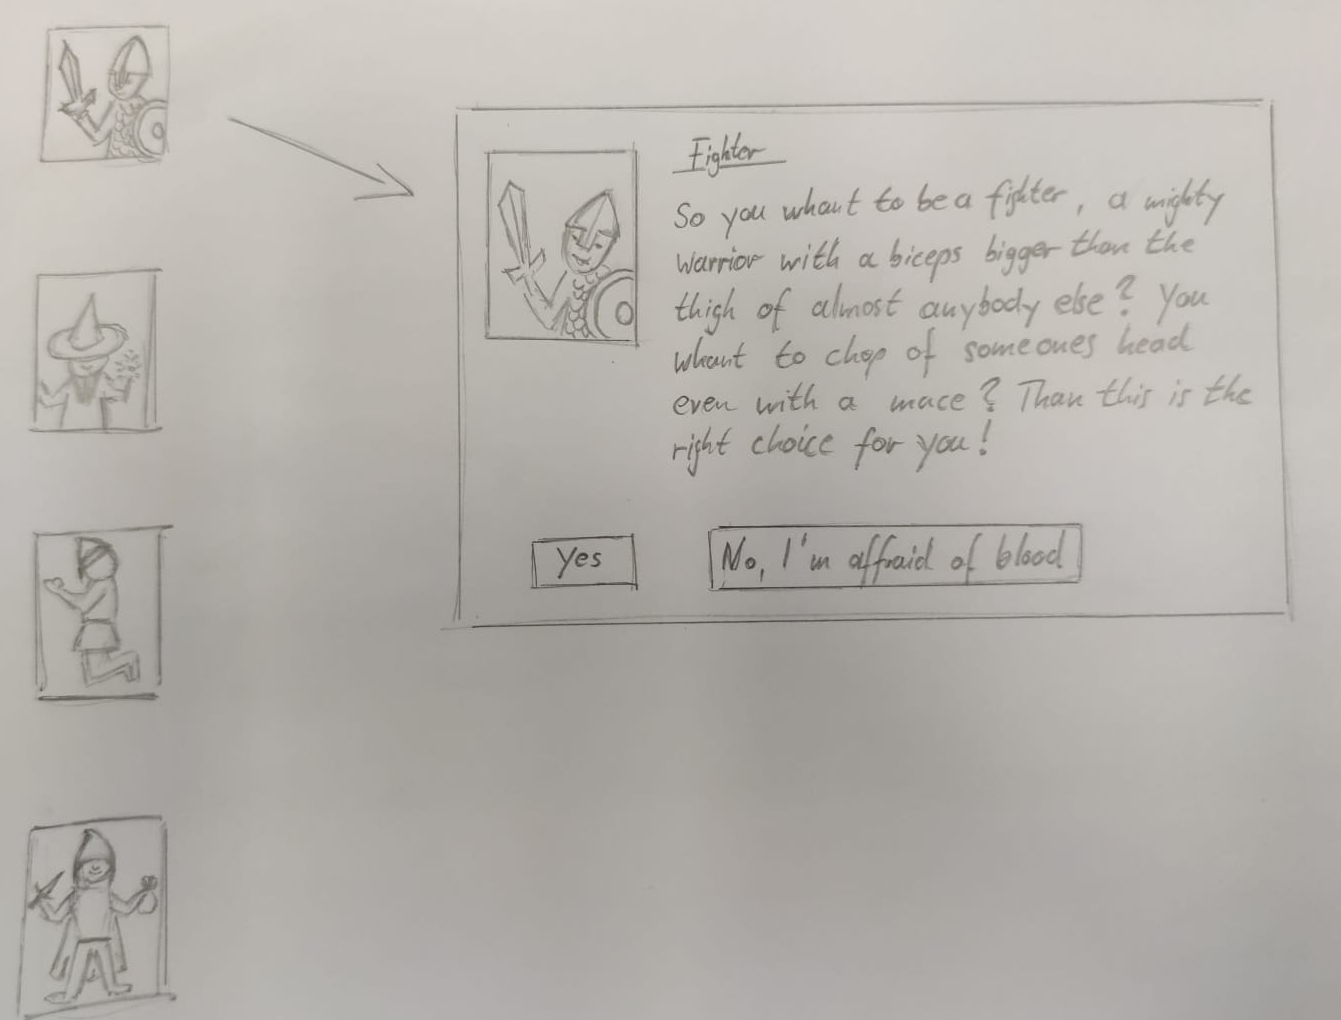
\includegraphics[width=1\textwidth]{2021-11-29-Entwurf-Klassen-Ui}
\end{figure}

2021-11-30-Entwurf-Lobby-Logik 
\begin{figure}[H]
    \centering
    \caption[]{2021-11-30-Entwurf-Lobby-Logik}
    \label{fig:2021-11-30-Entwurf-Lobby-Logik}
    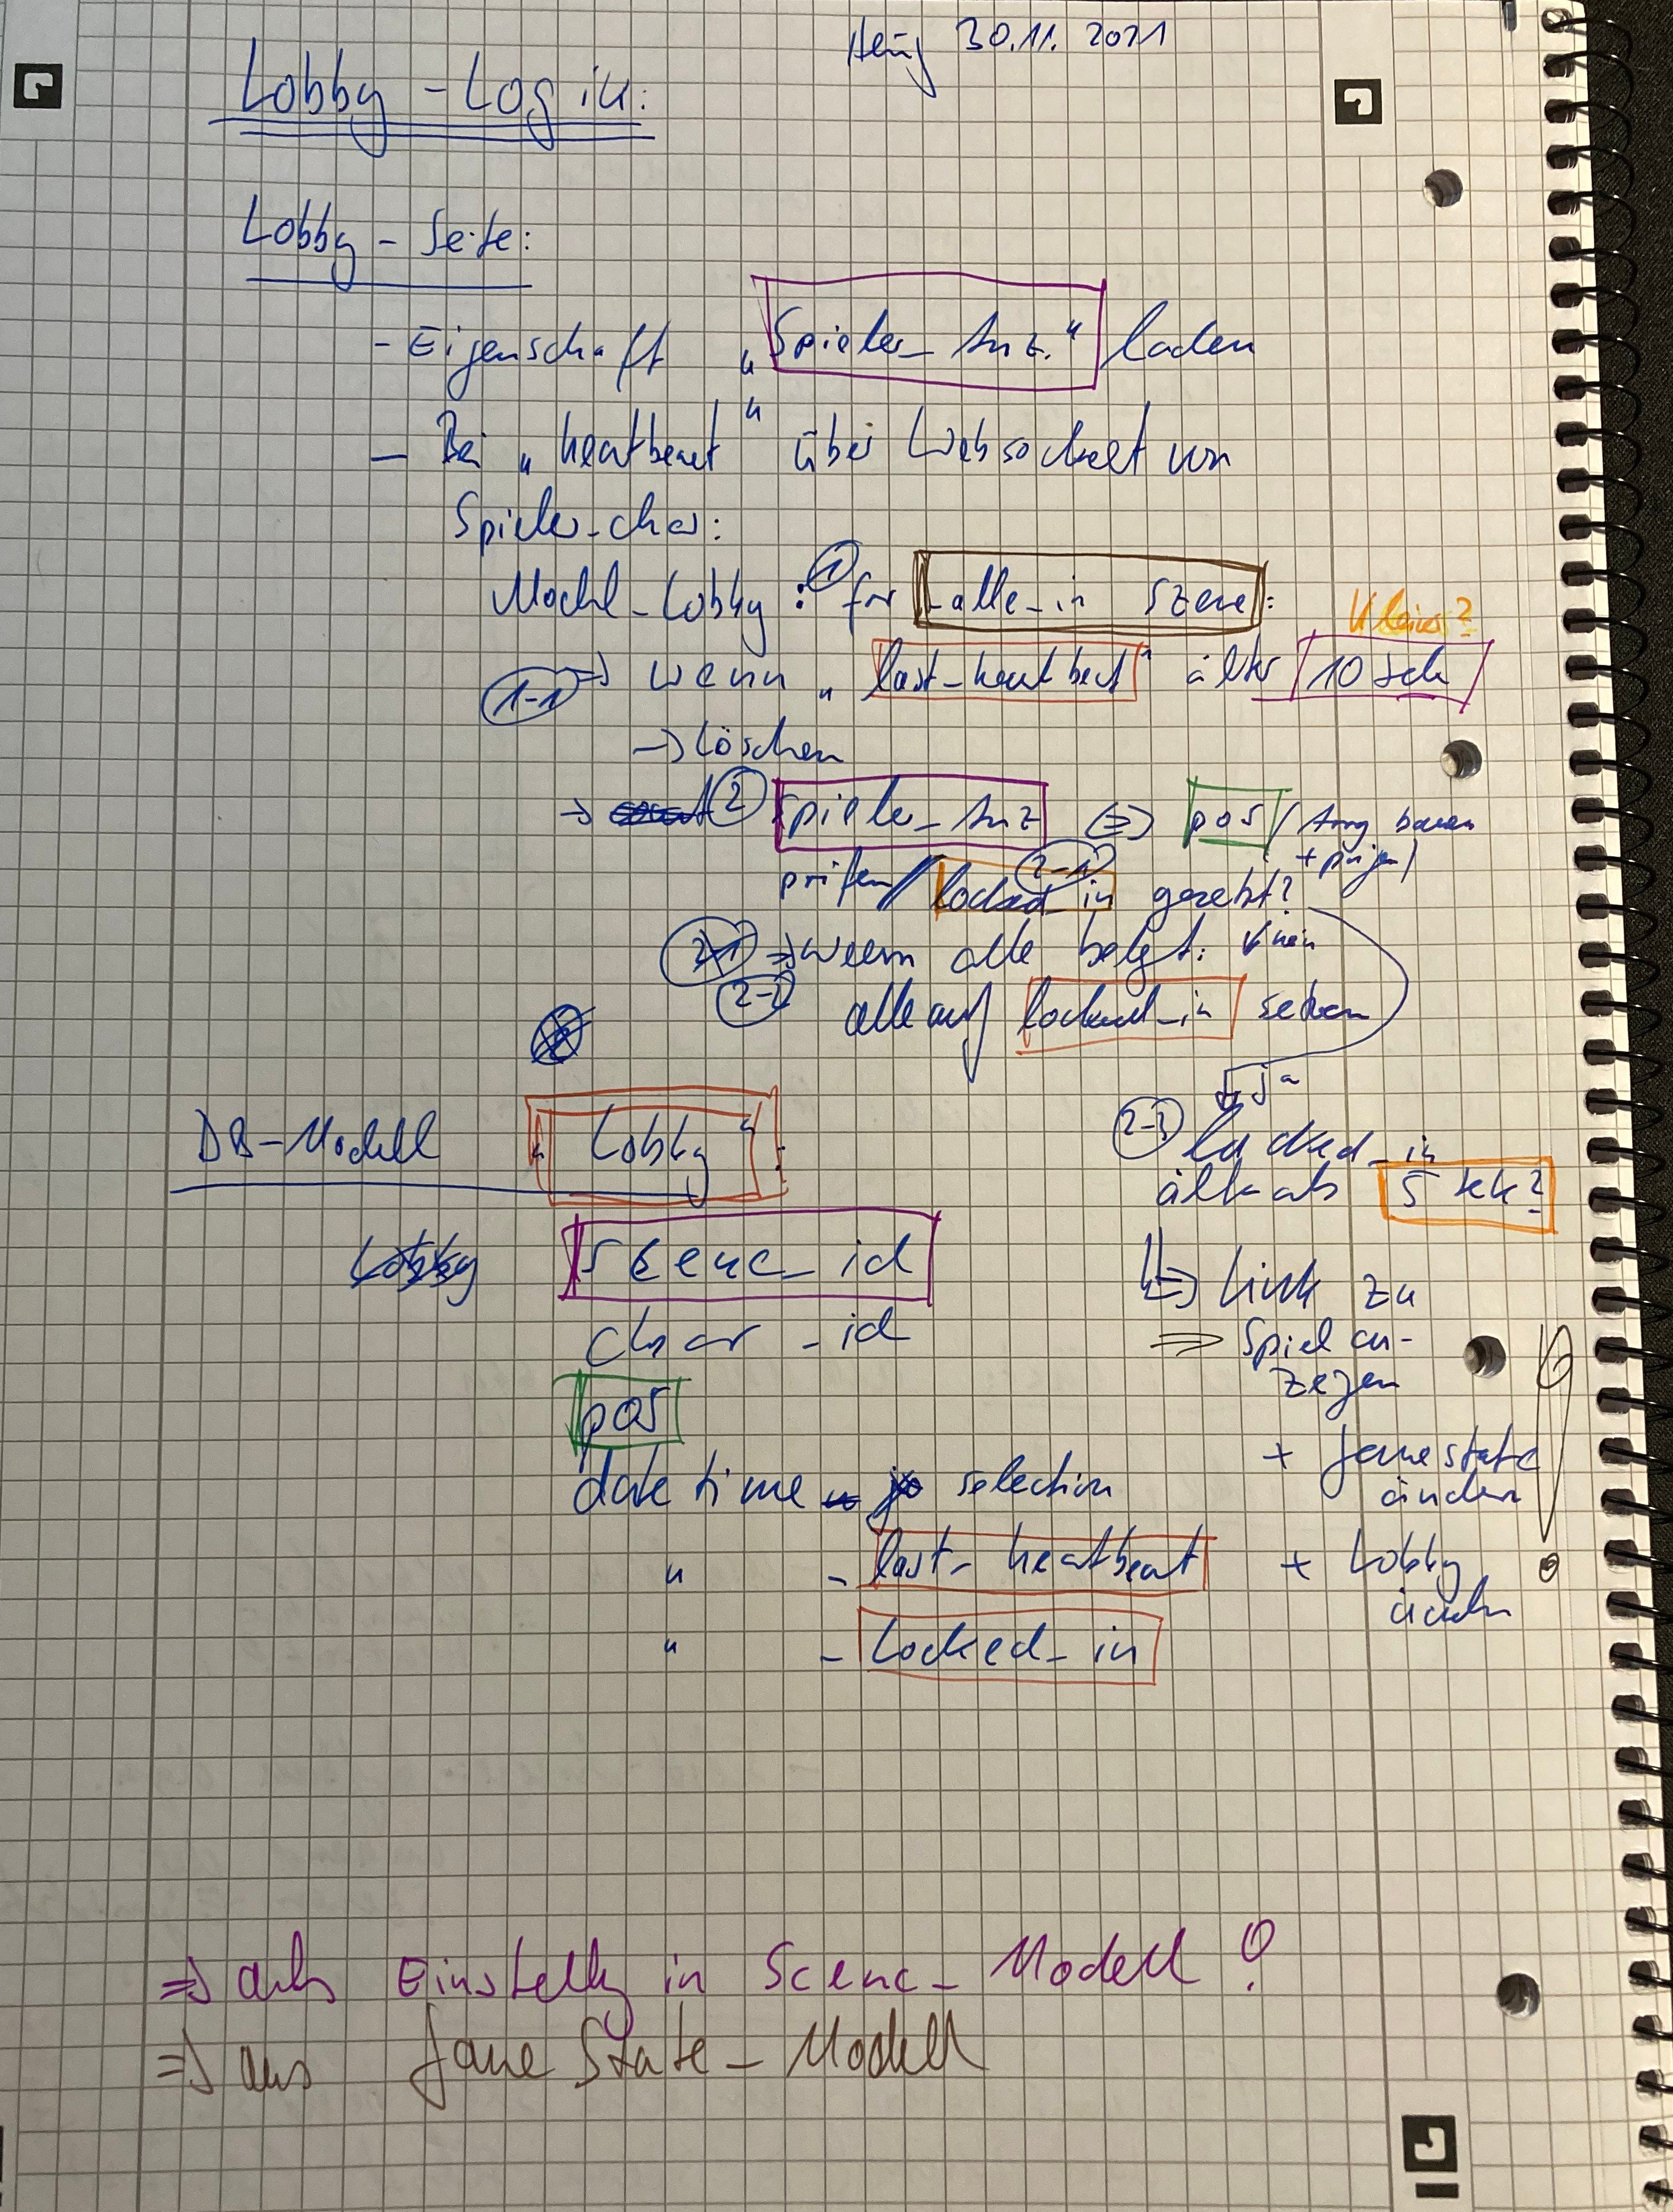
\includegraphics[width=1\textwidth]{2021-11-30-Entwurf-Lobby-Logik}
\end{figure}

2021-11-30-Entwurf-Lobby-UI 
\begin{figure}[H]
    \centering
    \caption[]{2021-11-30-Entwurf-Lobby-UI}
    \label{fig:2021-11-30-Entwurf-Lobby-UI}
    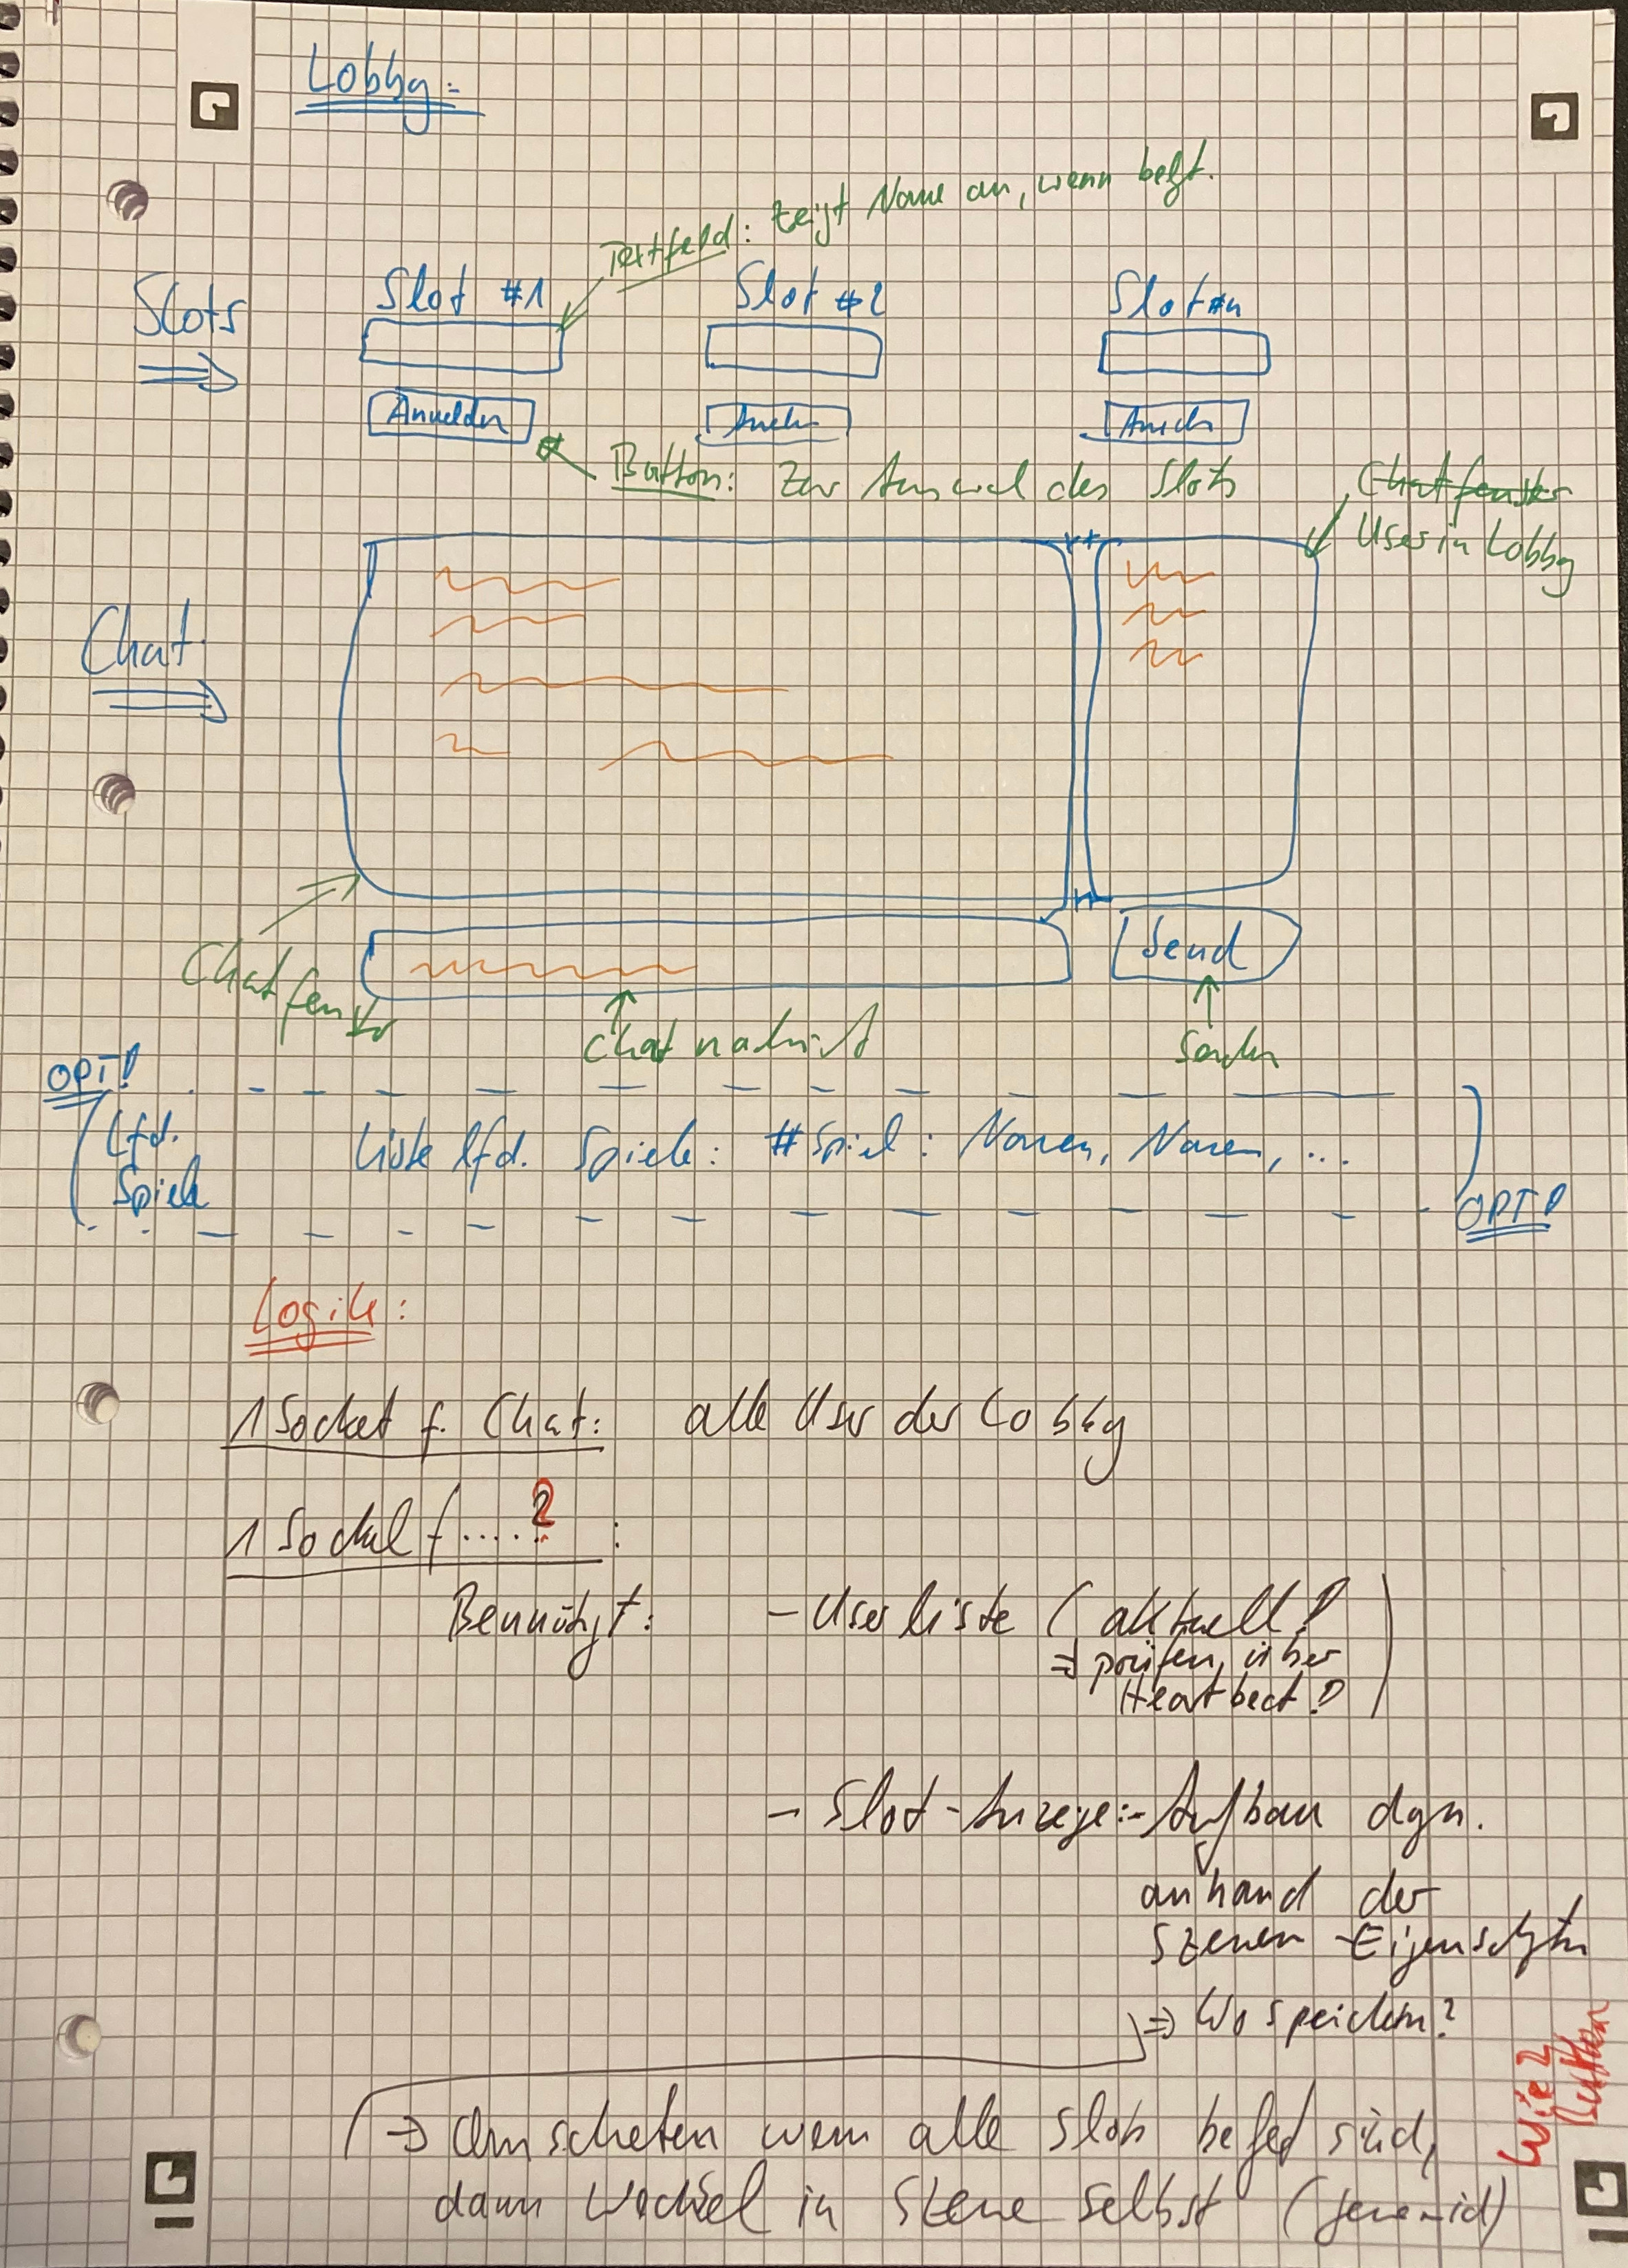
\includegraphics[width=1\textwidth]{2021-11-30-Entwurf-Lobby-UI}
\end{figure}

2021-12-02-Countdown-Logik 
\begin{figure}[H]
    \centering
    \caption[]{2021-12-02-Countdown-Logik}
    \label{fig:2021-12-02-Countdown-Logik}
    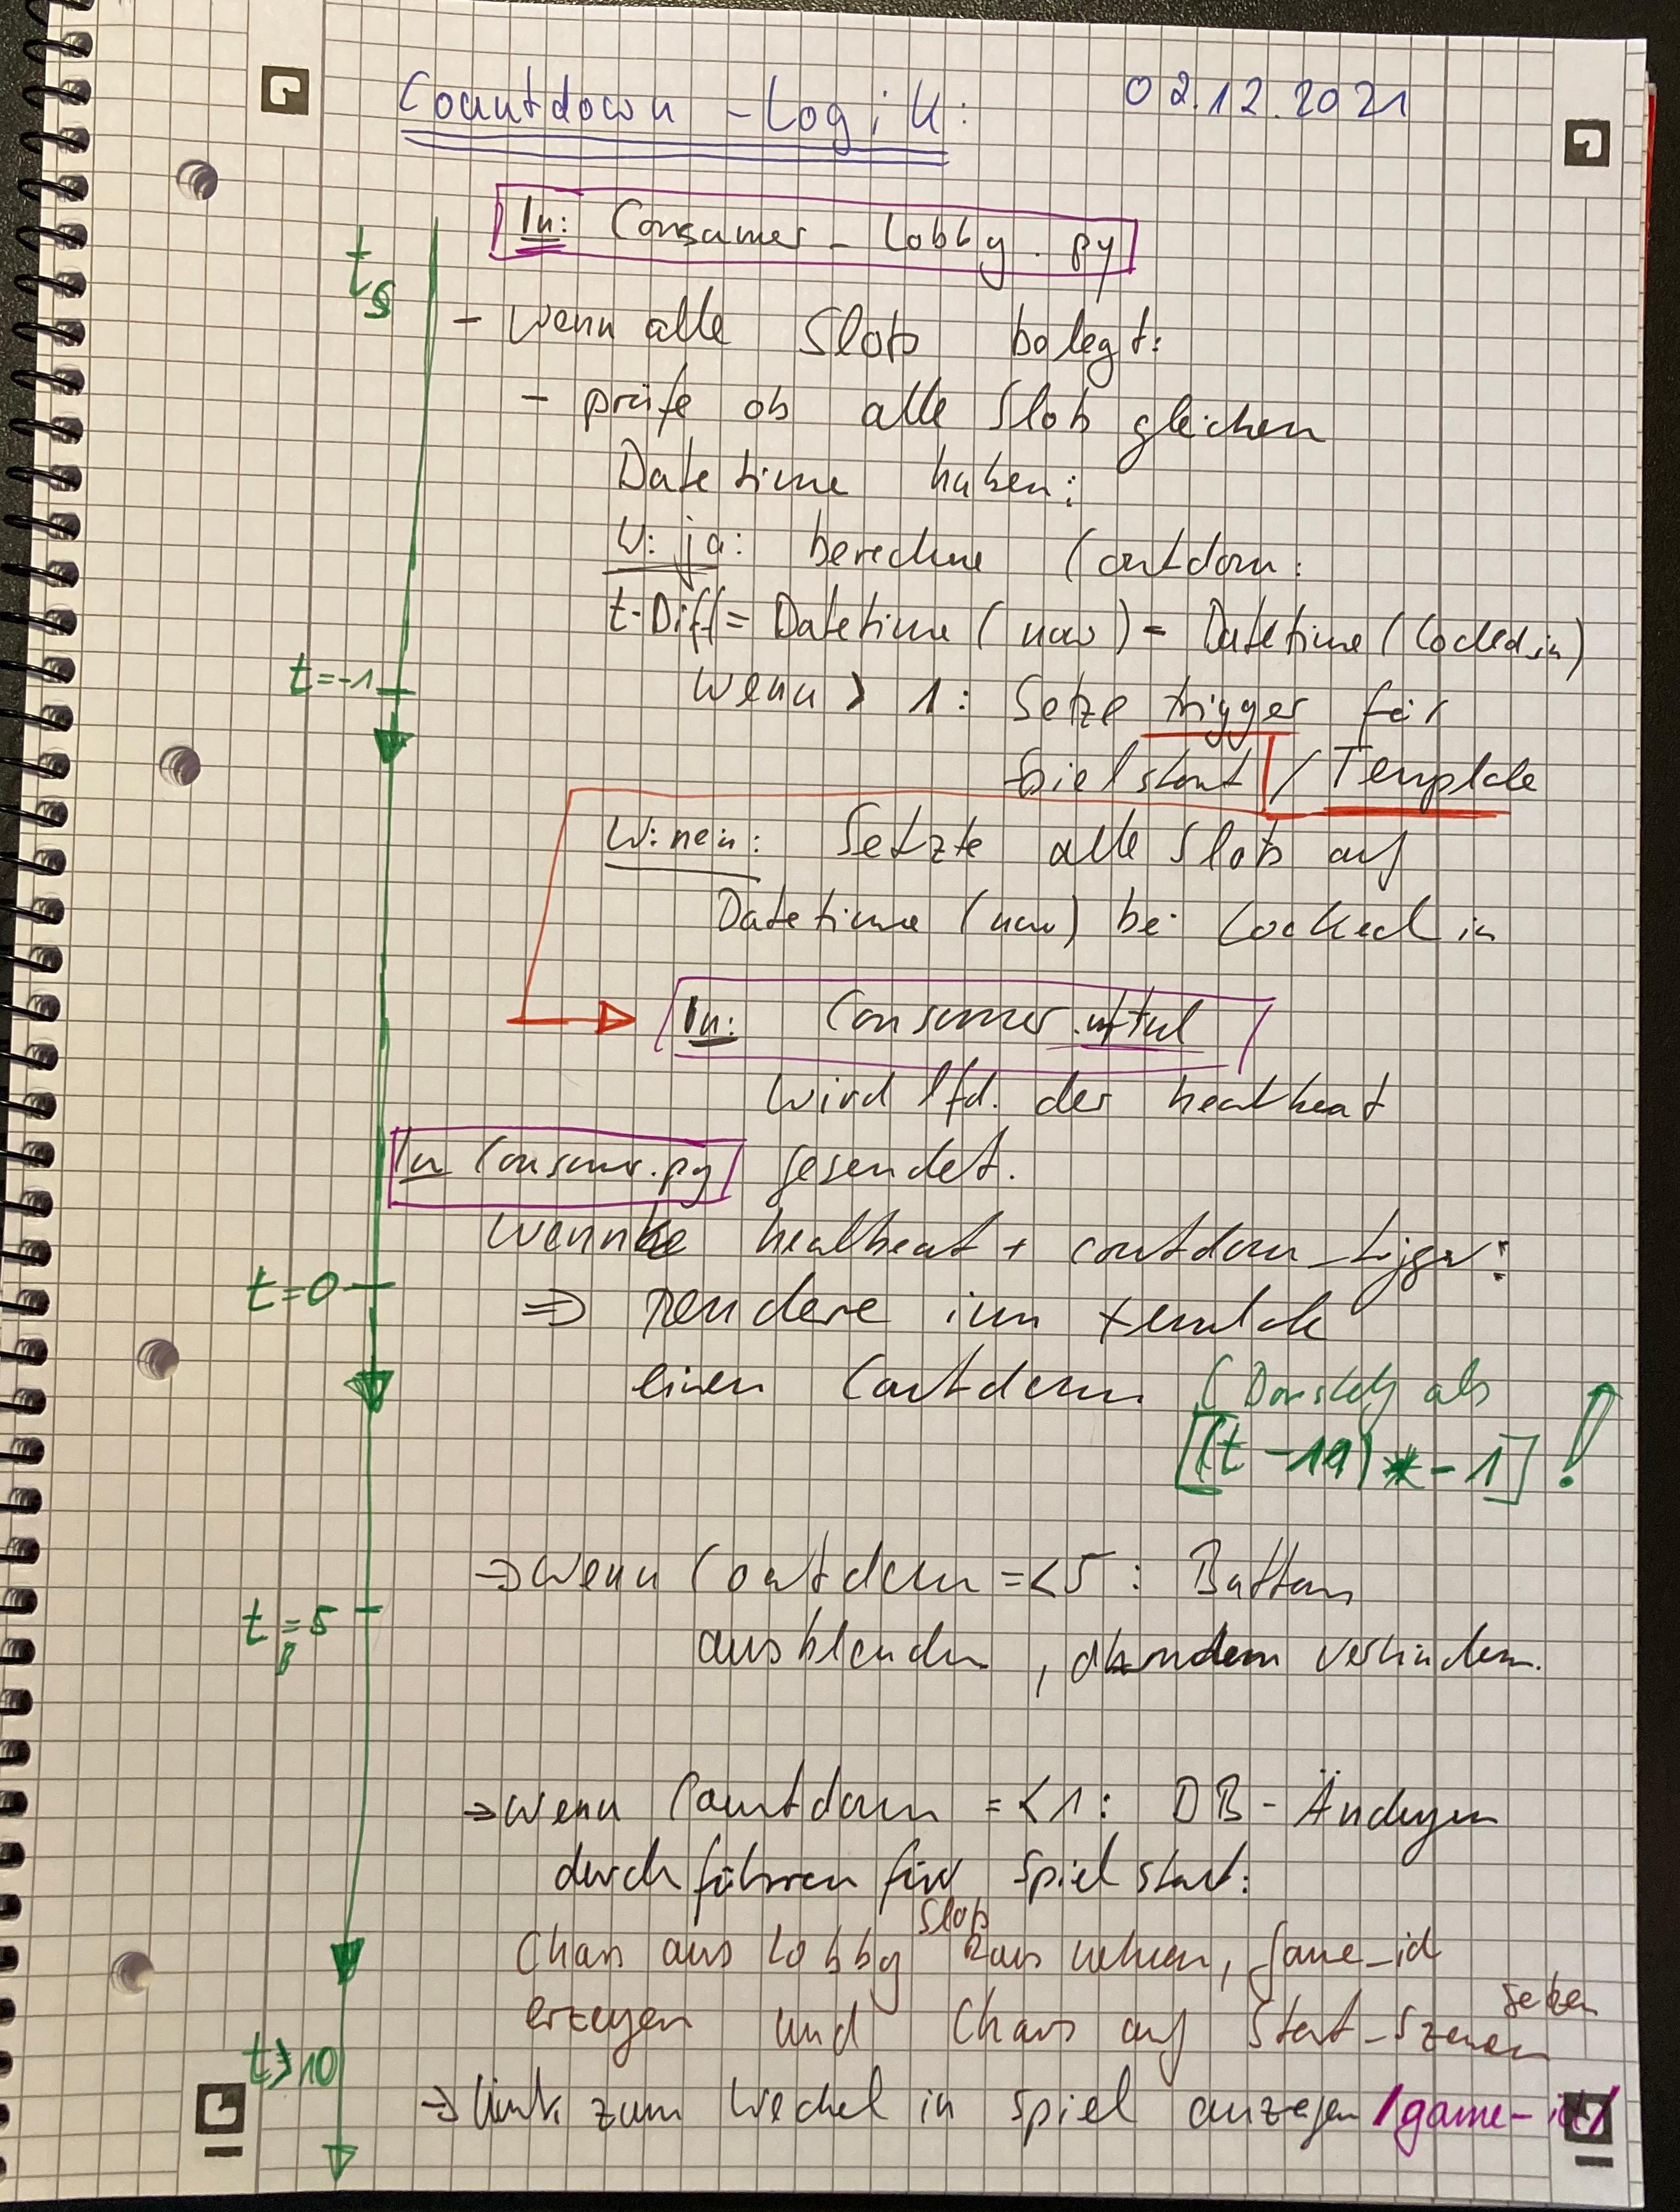
\includegraphics[width=1\textwidth]{2021-12-02-Countdown-Logik}
\end{figure}

2021-12-05-Projketbesprechung-Miro-b 
\begin{figure}[H]
    \centering
    \caption[]{2021-12-05-Projketbesprechung-Miro-b}
    \label{fig:2021-12-05-Projketbesprechung-Miro-b}
    
\includegraphics[width=1\textwidth]{2021-12-05-Projketbesprechung-Miro-b}
\end{figure}

2021-12-05-Projketbesprechung-Miro-c 
\begin{figure}[H]
    \centering
    \caption[]{2021-12-05-Projketbesprechung-Miro-c}
    \label{fig:2021-12-05-Projketbesprechung-Miro-c}
    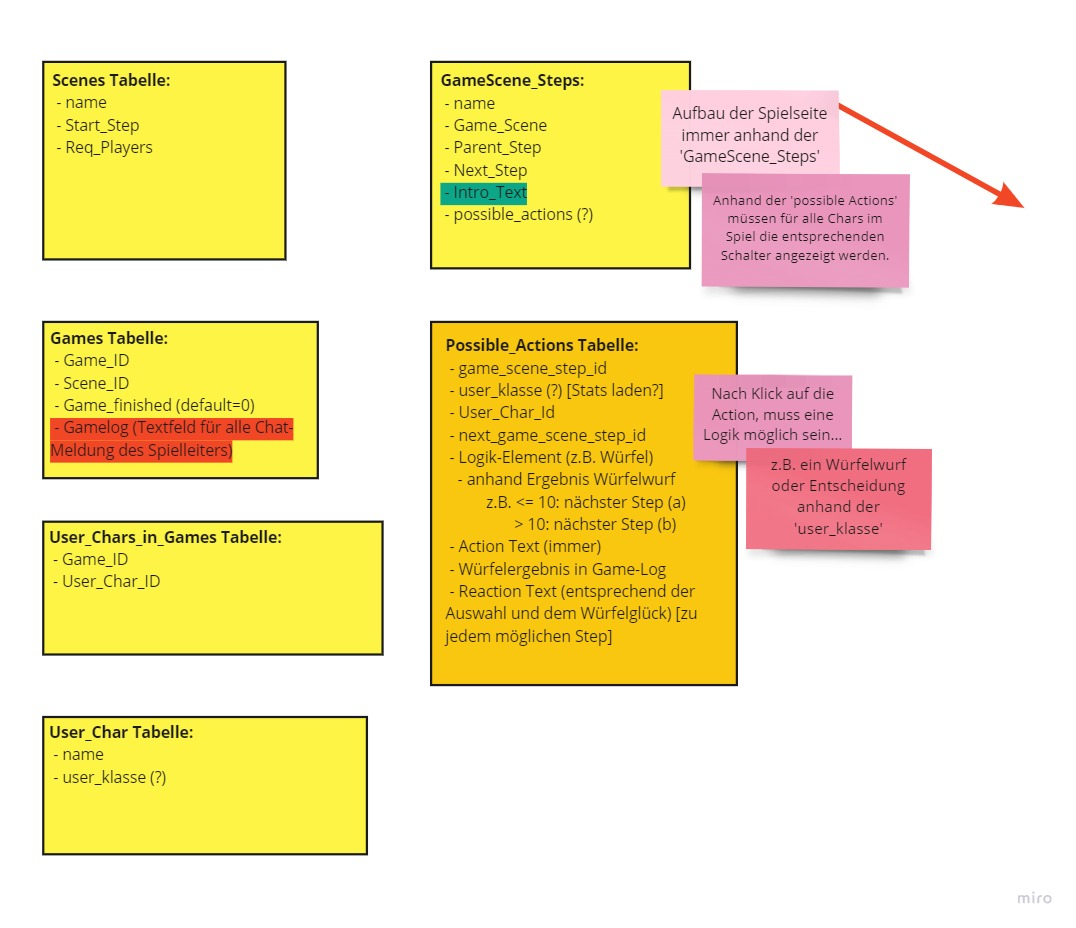
\includegraphics[width=1\textwidth]{2021-12-05-Projketbesprechung-Miro-c}
\end{figure}

2021-12-05-Projketbesprechung-Miro-d 
\begin{figure}[H]
    \centering
    \caption[]{2021-12-05-Projketbesprechung-Miro-d}
    \label{fig:2021-12-05-Projketbesprechung-Miro-d}
    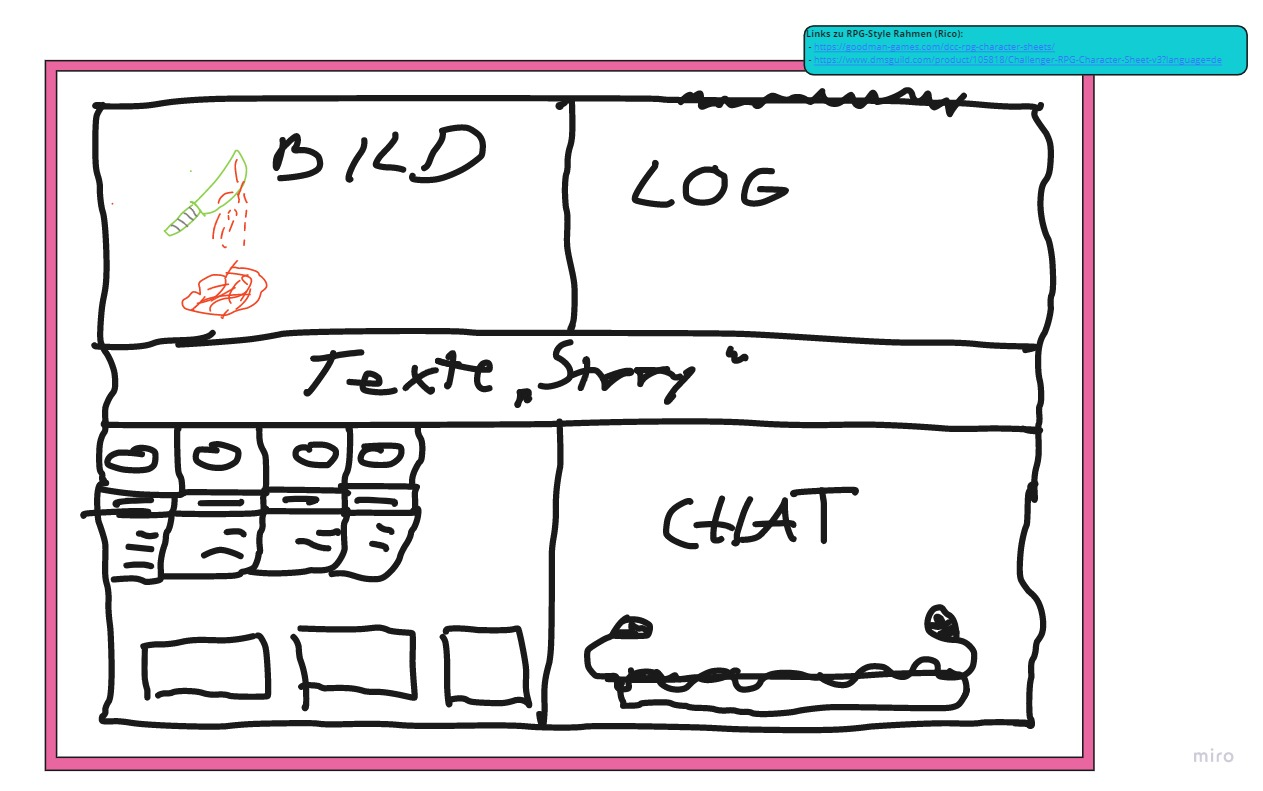
\includegraphics[width=1\textwidth]{2021-12-05-Projketbesprechung-Miro-d}
\end{figure}

2021-12-11-Projekt-Besprechung-Klassenbeschreibung 
\begin{figure}[H]
    \centering
    \caption[]{2021-12-11-Projekt-Besprechung-Klassenbeschreibung}
    \label{fig:2021-12-11-Projekt-Besprechung-Klassenbeschreibung}
    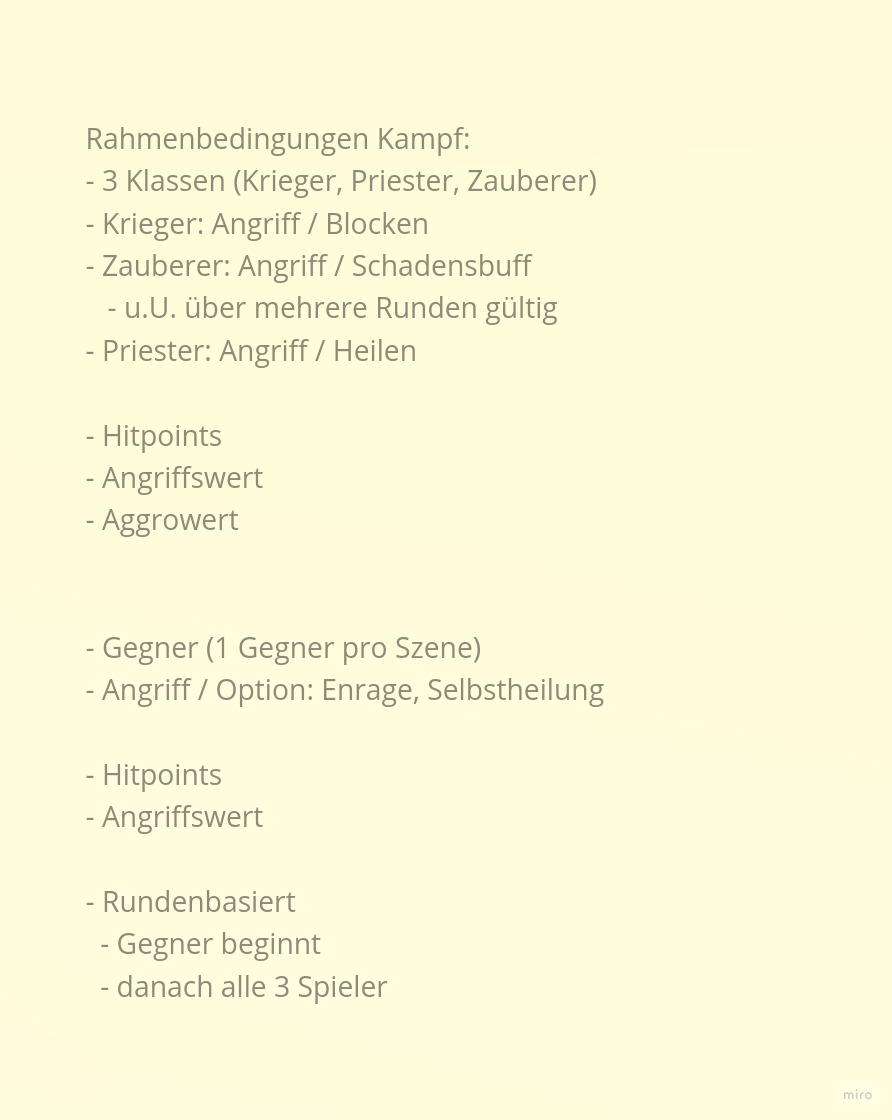
\includegraphics[width=1\textwidth]{2021-12-11-Projekt-Besprechung-Klassenbeschreibung}
\end{figure}


\begin{figure}[H]
    \centering
    \caption[]{11.12.2021: Projekt Besprechung: Gegenseitiges Update und Wechsel von Szenenlogik zu Kampfsystem für das RPG }
    \label{fig:2021-12-11-Projekt-Besprechung}
    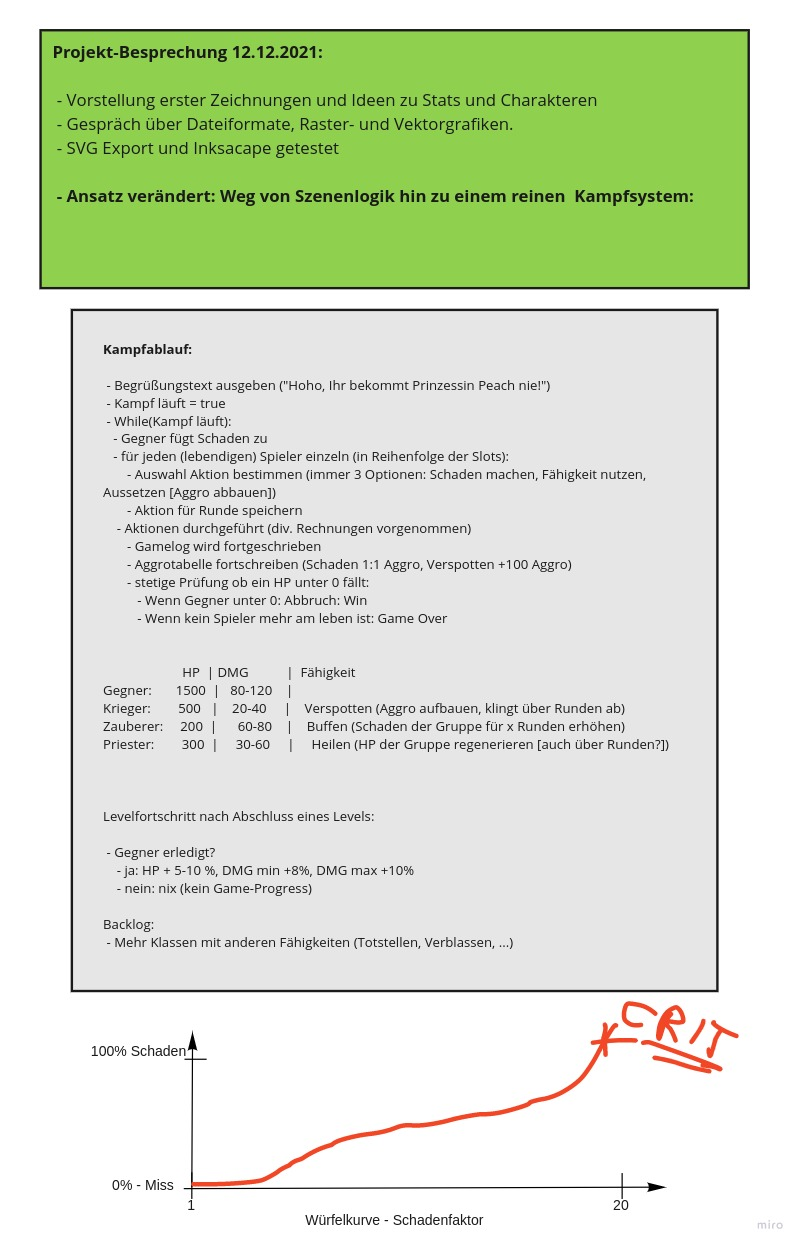
\includegraphics[width=1\textwidth]{2021-12-11-Projekt-Besprechung}
\end{figure}



\section{Entwicklungsnotizen}

\subsection{Entwicklung, Sonntag 19.12.2021:}

An diesem Tag wurden weitere, notwenige Grundlagen für die Integration der Spiellogik eingebaut. Das insbesondere in Vorbereitung auf die kommenden Anpassungen und Entwicklungen die in der Projektbesprechung vom 11.12.2021 besprochen wurden. 
Konkret: 

\begin{itemize}
	\item Prüfung auf den Seiten Chars, Worldmap und Lobby ob dieser Benutzer ein aktives Spiel hat. Falls ja, wird der Benutzer auf diese Seite umgeleitet.
	\item Grundfunktion für das Beenden von einem Spiel eingebaut: Man kann nun per Klick im Spiel, das Spiel beenden.
	\item Daran anschließend eine Prüfung im laufendem Spiel, ob das Spiele beendet wurde und falls ja, Anzeige eines Endbildschirms.
\end{itemize}

Die Entwicklung der Grundlagen an diesem Tag wurde mit Fokus auf Modularisierung erledigt. Der Code der jeweiligen Funktionen wurde in einzelnen Dateien ausgelagert um Wiederverwendbarkeit und Lesbarkeit zu erhöhen. 

Die zugehörigen Commits sind insbesondere: 
\url{https://git.io/JDjKl} und 
\url{https://git.io/JDjKB}


\subsection{Entwicklung, Dienstag 21.12.2021:}

Grundlagen des Kampfsystems entsprechend der Projekt-Besprechung vom 11.12.2021 (Abbildung \ref{fig:2021-12-11-Projekt-Besprechung}) sollen implementiert werden.

Vorbereitungen: 

\begin{itemize}
    \item Tabelle "GamesScenesSteps" und Verknüpfungen entfernen (Commits \url{https://git.io/JDjKz} und \url{https://git.io/JDjKg})
    \item Kampf-/Gamelog erzeugen: Darin werden alle Meldungen aus dem Spiel wie z.B. Kampftexte, Schaden, Aktionen, Systemmeldungen und alles andere denkbare angezeigt und gespeichert. Getrennt davon soll der Chat-Log dargestellt werden. Dazu werden in der Tabelle "Games" zwei neue Textfelder erzeugt (Commit \url{https://git.io/JDj63}). 
    \item Anzeige des Game-Logs auf der Spielseite. Schreiben von Nachrichten in das Gamelog als ersten Test des grundlegend umgestellten Seitenaufbaus: Es werden nur noch einzelene Elementinhalte per Websocket transportiert, nicht mehr ganze HTML-Code-Blöcke (Commit \url{https://git.io/JyeJQ}).
\end{itemize}


\subsection{Entwicklung, Montag 27.12.2021:} \label{ref-runden-impl}

Weitere Entwicklungen entsprechend der Projekt-Besprechung vom 11.12.2021 (Abbildung \ref{fig:2021-12-11-Projekt-Besprechung}):

\begin{itemize}
    \item Eintrag ins Gamelog zum Spielstart (Commit \url{https://git.io/JyBRf}).
    \item Rundensystem implementieren. Dazu mindestens notwendig: Lebens- und Angriffspunkte der User-Chars sowie des Gegners. 
    \begin{enumerate}
        \item Erster Schritt: Definition des Ablaufes einer Runde als Pseudo-Code: 
            \begin{enumerate}
                \item Gameloop-Schleife: [round-state]
                \item Aktion von Gegner ausführen (Schaden) [100]
                \item Prüfen ob User-Char tod ist (HP < 1 = Dead-Flag: True) [200]
                \item Prüfen wie viele User-Chars noch leben (n < 1 = Gameover-Flag: True, break-Gameloop-Schleife) [300]
                \item Aktionen der User-Chars aufnehmen (Entscheidung für nächste Aktion von jedem Spieler annehmen + wegspeichern) [400]
                \item Alle Aktionen der User-Chars ausführen (Aktionen laden und ausführen: Schaden, Aktion, Passen) [500]
                \item Nach jedem Spieler, prüfen ob Gegner besiegt wurde (HP < 1 = Win-Flag: True, break-Gameloop-Schleife) [immernoch 500]
                \item Rundencounter +1 [600]
                \item Gameloop-Schleife nächster Durchlauf [700, zurück zu 100]...
            \end{enumerate}
    Steuerung über "round-state" Hilfsvariable, gespeichert in Games-Tabelle (Default=0, Gameover=990, Win=995). Da der Aufruf der Spiele-Logik über den Websocket-Heartbeat der Spieler erfolgt, müssen die Arbeitsschritte sehr kleinteilig sein und diese laufend in kleinen (kleinsten?) Schritten weggepeichert werden. Möglicherweise ergibt sich ein Sync-Problem (Commit \url{https://git.io/JyRml})
    \item Zweiter Schritt: HP und AP bei User-Chars implementieren, damit AP aus "round-state 100: Gegner führt Schaden aus" durchgeführt werden kann (Commit \url{https://git.io/JyRWD}).  
    \end{enumerate}
\end{itemize}


\subsection{Entwicklung, Dienstag 28.12.2021:}

Fortführung der Entwicklungen vom Vortag. Hier insbesondere nun die Implementation der aller Funktionen der Runden- bzw. Spiellogik:

\begin{itemize}
    \item Auswahl eines zufälligen, lebenden Spielercharakters und zufügen von Schaden durch den Gegener. Außerdem Erweiterung Runden-/Gameloop und Fortschreiben des Game-Logs (Commit \url{https://git.io/JygDz}).
    \item Nächster Rundenschritt 200: Prüfen ob Spieler gestorben sind und Meldung im Game-Log ausgeben falls in aktueller Runde gestorben (Commit \url{https://git.io/Jya3H}). 
\end{itemize}


\subsection{Entwicklung, Mittwoch 29.12.2021:}

Weitere Implementation von Rundenlogik:

\begin{itemize}
    \item Rundenschritt 300: Feststellen ob alle Spieler verstorben sind, falls ja in Spielende springen (Commit \url{https://git.io/Jy1Lu}).
    \item Tests ergaben Probleme beim Spiel mit mehreren Spielern. Die Rundenlogik wird dann gleichzeitig vorangetrieben. Dadurch werden manche Aktionen und Rundenschritte mehrfach ausgeführt. Ein Versuch das Problem mit einem Token (ähnlich einem Semaphor) zu lösen, brachte leider noch keinen abschließenden Erfolg. Der Singleplayer aber, geht fehlerfrei. Das Problem wird daher zurückgestellt und nun zuerst die Entwicklung weiterer Punkte fortgeführt (Commit \url{https://git.io/Jy1qZ}).
    \item Als Workaround für oben genanntes Problem im Mulitplayer wurde nun eingestellt, dass immer nur der erste Spieler eines Spiels die Rundenlogik vorantreibt. Das ist etwas mehr fehleranfällig als eine korrekte Tokenlösung, wird für das Projekt hier aber vorerst ausreichend sein (Commit \url{https://git.io/Jy1su}).
    \item Umfangreiche Erweiterungen und Anpassungen für das Anzeigen der User-Chars auf der Spieleseite, darstellen und aussteuern der Aktions-Buttons, das einsammeln der Aktionen in der Datenbank und ebenso bereits das zurücksetzen beim Rundenwechsel (Commit \url{https://git.io/JyDlp}).

    \begin{figure}[H]
        \centering
        \caption[]{29.12.2021: Bildschirmfoto zum Entwicklungsstand mit Runden-Status 400.}
        \label{fig:2021-12-29-Bildschirmfoto-Entwicklungsstand-Runden-Status-400.png}
        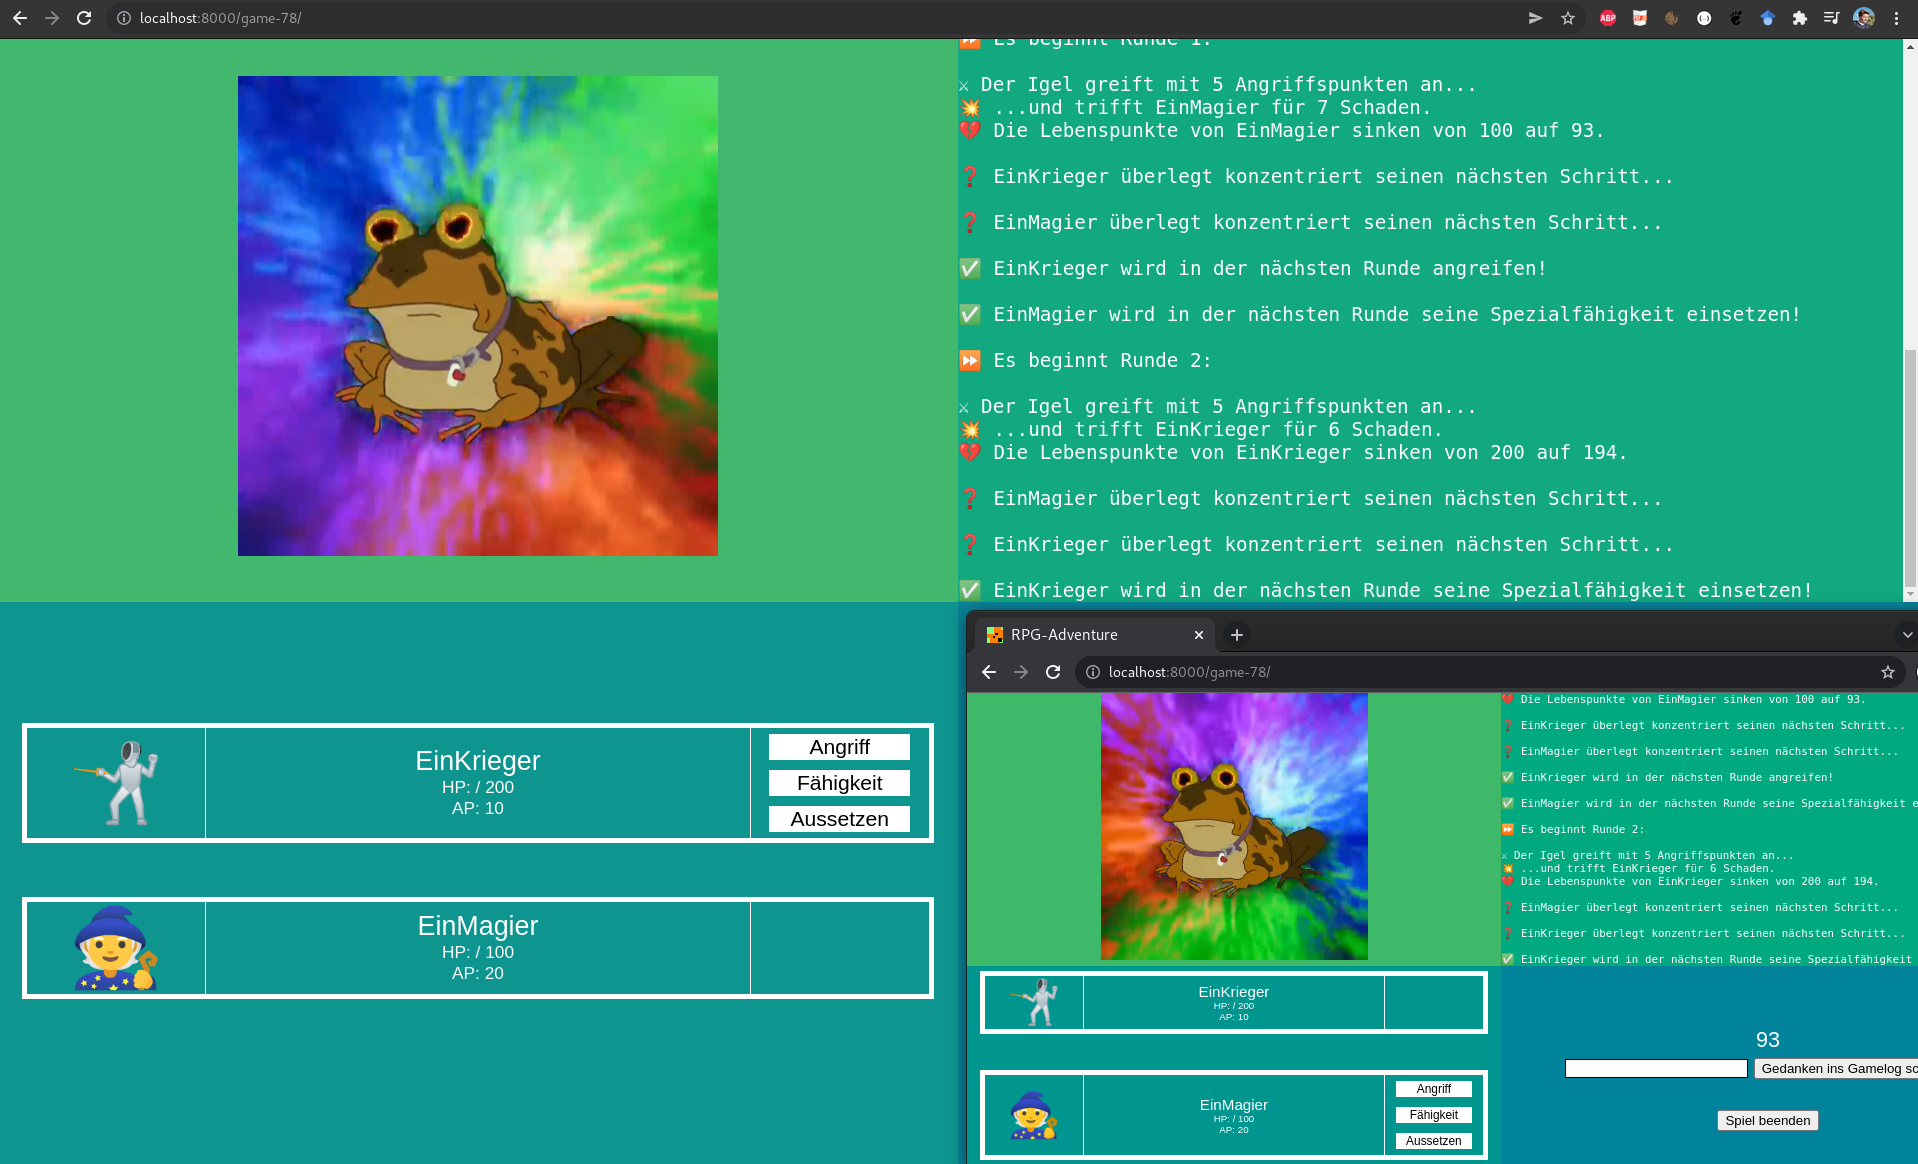
\includegraphics[width=0.7\textwidth]{2021-12-29-Bildschirmfoto-Entwicklungsstand-Runden-Status-400.png}
    \end{figure}

    \item Die Chatfunktion wurde implementiert. Hier jedoch abweichend vom Plan direkt als Meldungen im Game-Log und nicht in einem gesonderten Chat-Log und Chat-Fenster. Julian war damit im kurzen Teams-Gespräch gestern einverstanden. Den Aufbau der Game-Seite entsprechend angepasst und dem Game-Log deutlich mehr Raum eingeräumt. Außerdem weitere Anpassungen am Design und Style (Commit \url{https://git.io/JyDRK}).

\end{itemize}


\subsection{Entwicklung, Donnerstag 30.12.2021:}

Abschließender Schritt in der Implementation der Rundenlogik:

\begin{itemize}
    \item Die Schadensfunktion für Spieler wurde eingebaut: Damit kann dem Gegner nun Schaden zugefügt werden. Außerdem Prüfung auf Tod des Gegners incl. entsprechender Medlung (Commit \url{https://git.io/Jy9E7}).
\end{itemize}

Offen sind nun als nächste Schritte noch:
\begin{enumerate}
    \item Fähigkeiten der Spieler in Rundenlogik implementieren.
    \item Abschlussbildschirm für Win und Gameover konzeptionieren und implementieren. 
    \item Charakterentwicklung bei Win implementieren.
    \item Würfel bei Schaden bzw. Angriff implementieren.
    \item Aggrotabelle und verbundene Funktionen implementieren.
\end{enumerate}



\section{Noitzen für Reflektion}

\subsection{Rundenbasierter vs. chaotischer Spielablauf}

Der Ansatz die Entwicklung durch den Einsatz eines rundenbasierten Ablaufs bzw. Kampfsystems deutlich zu vereinfachen, muss wohl nach den Entwicklungen vom 27.12.2021 (\ref{ref-runden-impl}) zumindest angezweifelt werden. Denn der Aufwand, der durch die dadurf notwendige Konzeptionierung und Detailplanung entsteht ist nicht zu unterschätzen. Demengegen stünde bei einem chaotischen Spielablauf lediglich das Handling der Events. 

\subsection{Kleinteilige Aufgabenpakete} 

In der Entwicklung eine überschaubare Anzahl an kleinteiligen bzw. Teilufgaben vor sich zu haben, empfinde ich als sehr hilfreich. Man hat damit einen Überblick über die Arbeit der nächsten Tage. Bei der Entwicklung der Rundenlogik hatte ich durch die Kenntniss um die nächsten Runden-Schritte hier einen guten Überblick. Der Abschluss jeder einzelnen Teil-Aufgabe sorgte da laufend für postive Motivation. 
Ich vermute, dass dieser Effekt sehr ähnlich bei den agilen Methoden zum tragen kommt und zur Motivation genutzt wird. 

\subsection{Stichwortsammlung für Refektion}

\begin{itemize}
    \item Projektaufteilung: So abstimmen, dass verschiedene Arbeitsschritte gleichzeitig von verschiedenen Personen bearbeitet werden können.  
\end{itemize}
